
\documentclass{article}

% -----------------------------
% Packages
% -----------------------------
\usepackage{fancyhdr}
\usepackage{extramarks}
\usepackage{amsmath}
\usepackage{amsthm}
\usepackage{amsfonts}
\usepackage{tikz}
\usepackage[plain]{algorithm}
\usepackage{algpseudocode}
\usepackage{amssymb}
\usepackage{graphicx}

\usetikzlibrary{automata,positioning}

% -----------------------------
% Basic Document Settings
% -----------------------------
\topmargin=-0.45in
\evensidemargin=0in
\oddsidemargin=0in
\textwidth=6.5in
\textheight=9.0in
\headsep=0.25in

\linespread{1.1}

\pagestyle{fancy}
\lhead{\hmwkAuthorName}
\chead{\hmwkClass: \hmwkTitle}
\rhead{}
\lfoot{\lastxmark}
\cfoot{\thepage}

\renewcommand\headrulewidth{0.4pt}
\renewcommand\footrulewidth{0.4pt}

\setlength\parindent{0pt}

% -----------------------------
% Problem Section Helpers
% -----------------------------
\newcommand{\enterProblemHeader}[1]{
  \nobreak\extramarks{}{Problem \arabic{#1} continued on next page\ldots}\nobreak{}
  \nobreak\extramarks{Problem \arabic{#1} (continued)}{Problem \arabic{#1} continued on next page\ldots}\nobreak{}
}

\newcommand{\exitProblemHeader}[1]{
  \nobreak\extramarks{Problem \arabic{#1} (continued)}{Problem \arabic{#1} continued on next page\ldots}\nobreak{}
  \stepcounter{#1}
  \nobreak\extramarks{Problem \arabic{#1}}{}\nobreak{}
}

\setcounter{secnumdepth}{0}
\newcounter{partCounter}
\newcounter{homeworkProblemCounter}
\setcounter{homeworkProblemCounter}{1}
\nobreak\extramarks{Problem \arabic{homeworkProblemCounter}}{}\nobreak{}

% -----------------------------
% Theorem env (optional)
% -----------------------------
\newtheorem*{theorem}{Theorem}

% -----------------------------
% Homework Problem Environment
%   Usage:
%   \begin{homeworkProblem}            % auto-number
%     % Your answer here
%   \end{homeworkProblem}
%
%   \begin{homeworkProblem}[7]         % set problem number to 7
%     % Your answer here
%   \end{homeworkProblem}
% -----------------------------
\newenvironment{homeworkProblem}[1][-1]{
  \ifnum#1>0
    \setcounter{homeworkProblemCounter}{#1}
  \fi
  \section{Problem \arabic{homeworkProblemCounter}}
  \setcounter{partCounter}{1}
  \enterProblemHeader{homeworkProblemCounter}
}{
  \exitProblemHeader{homeworkProblemCounter}
}

% -----------------------------
% Homework Details (EDIT THESE)
% -----------------------------
\newcommand{\hmwkTitle}{Homework \ 1}
\newcommand{\hmwkClass}{CS 4262}
\newcommand{\hmwkClassInstructor}{Prof. Dr. Thomas Beckers}
\newcommand{\hmwkAuthorName}{\textbf{Joseph Quinn}}

% -----------------------------
% Title
% -----------------------------
\title{
  \vspace{2in}
  \textmd{\textbf{\hmwkClass:\ \hmwkTitle}}\\
  \vspace{0.1in}\large{\textit{\hmwkClassInstructor\ }}
  \vspace{3in}
}
\author{\hmwkAuthorName}
\date{}

% -----------------------------
% Convenience Macros (optional)
% -----------------------------
\renewcommand{\part}[1]{\textbf{\large Part \Alph{partCounter}}\stepcounter{partCounter}\\}

% Algorithms
\newcommand{\alg}[1]{\textsc{\bfseries \footnotesize #1}}

% Calculus
\newcommand{\deriv}[1]{\frac{\mathrm{d}}{\mathrm{d}x} (#1)}
\newcommand{\pderiv}[2]{\frac{\partial}{\partial #1} (#2)}
\newcommand{\dx}{\mathrm{d}x}

% Statistics
\newcommand{\E}{\mathrm{E}}
\newcommand{\Var}{\mathrm{Var}}
\newcommand{\Cov}{\mathrm{Cov}}
\newcommand{\Bias}{\mathrm{Bias}}

% Proof step (for aligned derivations)
\newcommand{\step}[2]{& #1 & & \text{#2} \\}

% Solution header (optional)
\newcommand{\solution}{\textbf{\large Solution}}

% -----------------------------
% Document
% -----------------------------
\begin{document}

\maketitle
\pagebreak

\begin{homeworkProblem}
	\subsection{Part 1}
	\textbf{(a) Conditional distribution.}
	\[
		p(y^{(i)} \mid x^{(i)} , f, \sigma)
		= \frac{1}{\sqrt{2\pi\sigma^2}}
		\exp\!\left( -\frac{\big(y^{(i)} - f(x^{(i)} )\big)^2}{2\sigma^2} \right).
	\]

	\textbf{(b) Log-likelihood.}

	First write the likelihood of all $N$ data points:
	\[
		L(f) = \prod_{i=1}^N p\!\big(y^{(i)} \mid x^{(i)}, f, \sigma\big).
	\]

	Taking logs:
	\begin{align*}
		\ell(f) & = \log L(f)                                                      \\
		        & = \sum_{i=1}^N \log p\!\big(y^{(i)} \mid x^{(i)}, f, \sigma\big) \\
		        & = \sum_{i=1}^N \left[
			-\tfrac{1}{2}\log(2\pi\sigma^2)
			- \tfrac{1}{2\sigma^2}\big(y^{(i)} - f(x^{(i)})\big)^2
		\right]                                                                    \\
		        & = -\frac{N}{2}\log(2\pi\sigma^2)
		- \frac{1}{2\sigma^2}\sum_{i=1}^N \big(y^{(i)} - f(x^{(i)})\big)^2.
	\end{align*}

	\textbf{(c) Analytic MLE for $c$.}

	Assume $f(x^{(i)}) = \phi(x^{(i)})^\top c$ with
	\[
		c =
		\begin{bmatrix}
			c_0 \\ c_1 \\ c_2
		\end{bmatrix}.
	\]

	Maximizing $\ell(f)$ is equivalent to minimizing the sum of squared errors:
	\[
		\hat c = \arg\min_c \sum_{i=1}^N \big(y^{(i)} - \phi(x^{(i)})^\top c\big)^2.
	\]

	Writing in matrix form with $X \in \mathbb{R}^{N \times 3}$
	(rows $\phi(x^{(i)})^\top$) and $y \in \mathbb{R}^N$:
	\[
		\hat c = \arg\min_c \|y - Xc\|_2^2
		\quad \Rightarrow \quad
		\hat c = (X^\top X)^{-1}X^\top y.
	\]
\end{homeworkProblem}
\pagebreak
\subsection{Part 2}

\textbf{(a) Conditional distribution.}

Now the noise variance depends on $i$, with
\[
	\varepsilon^{(i)} \sim \mathcal{N}(0, (\sigma^{(i)})^2).
\]
Thus,
\[
	p(y^{(i)} \mid x^{(i)}, f, \sigma^{(i)})
	= \frac{1}{\sqrt{2\pi(\sigma^{(i)})^2}}
	\exp\!\left( -\frac{\big(y^{(i)} - f(x^{(i)})\big)^2}{2(\sigma^{(i)})^2} \right).
\]

\textbf{(b) Log-likelihood.}

The full likelihood is
\[
	L(f) = \prod_{i=1}^N p\!\big(y^{(i)} \mid x^{(i)}, f, \sigma^{(i)}\big).
\]

Taking logs:
\begin{align*}
	\ell(f) & = \log L(f)                                                            \\
	        & = \sum_{i=1}^N \log p\!\big(y^{(i)} \mid x^{(i)}, f, \sigma^{(i)}\big) \\
	        & = \sum_{i=1}^N \left[
		-\tfrac{1}{2}\log(2\pi (\sigma^{(i)})^2)
		- \tfrac{1}{2(\sigma^{(i)})^2}\big(y^{(i)} - f(x^{(i)})\big)^2
		\right].
\end{align*}

\textbf{(c) Analytic MLE for $c$.}

As before, assume $f(x^{(i)}) = \phi(x^{(i)})^\top c$ with
\[
	c =
	\begin{bmatrix}
		c_0 \\ c_1 \\ c_2
	\end{bmatrix}.
\]

Maximizing $\ell(f)$ is equivalent to minimizing the weighted squared error:
\[
	\hat c = \arg\min_c \sum_{i=1}^N \frac{1}{(\sigma^{(i)})^2}
	\big(y^{(i)} - \phi(x^{(i)})^\top c\big)^2.
\]

Define the weights
\[
	\alpha^{(i)} = \frac{1}{(\sigma^{(i)})^2},
\]
and the diagonal weight matrix
\[
	A = \mathrm{diag}\!\big(\alpha^{(1)}, \alpha^{(2)}, \ldots, \alpha^{(N)}\big).
\]

Then, in matrix form with $X \in \mathbb{R}^{N \times 3}$ and $y \in \mathbb{R}^N$,
\[
	\hat c = (X^\top A X)^{-1} X^\top A y.
\]
\pagebreak
\subsection{Part 3}

\textbf{(a) Conditional distribution.}

The noise terms follow a Laplace distribution with location $\mu = 0$ and scale $b$.
Since $y^{(i)} = f(x^{(i)}) + \varepsilon^{(i)}$, we have
\[
	p(y^{(i)} \mid x^{(i)}, f, b)
	= \frac{1}{2b} \exp\!\left(
	-\frac{\big|y^{(i)} - f(x^{(i)})\big|}{b}
	\right).
\]

\textbf{(b) Log-likelihood.}

The likelihood is
\[
	L(f) = \prod_{i=1}^N p\!\big(y^{(i)} \mid x^{(i)}, f, b\big).
\]

Taking logs:
\begin{align*}
	\ell(f) & = \log L(f)                                                     \\
	        & = \sum_{i=1}^N \log \left[
	\frac{1}{2b} \exp\!\left(
	-\frac{|y^{(i)} - f(x^{(i)})|}{b}
	\right)
	\right]                                                                   \\
	        & = \sum_{i=1}^N \left[
	-\log(2b) - \frac{|y^{(i)} - f(x^{(i)})|}{b}
	\right]                                                                   \\
	        & = -N \log(2b) - \frac{1}{b}\sum_{i=1}^N |y^{(i)} - f(x^{(i)})|.
\end{align*}

\textbf{(c) Robustness.}

Maximizing $\ell(f)$ is equivalent to minimizing the sum of absolute deviations:
\[
	\hat f = \arg\min_f \sum_{i=1}^N |y^{(i)} - f(x^{(i)})|.
\]

This is the \emph{least absolute deviations} (L1) regression problem.
Compared to least squares (L2), the L1 loss grows linearly rather than quadratically,
so large errors (outliers) have less influence.
This makes the estimator more robust to outliers in the data.
\pagebreak
\begin{homeworkProblem}
	\subsection{Part 1}
	\textbf{(x1)}
	Error: 53,007.39
	\begin{figure}[h] % h = here, t = top, b = bottom
		\centering
		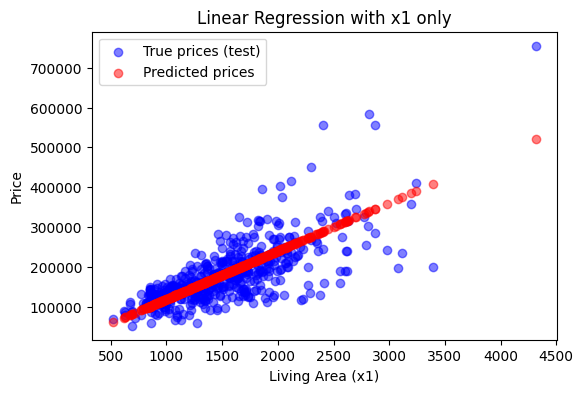
\includegraphics[width=0.6\textwidth]{../imgs/model_x1.png} % 
		\caption{Linear regression fit (x1)}
	\end{figure}

	\textbf{(x2)}
	Error: 67,402.18
	\begin{figure}[h] % h = here, t = top, b = bottom
		\centering
		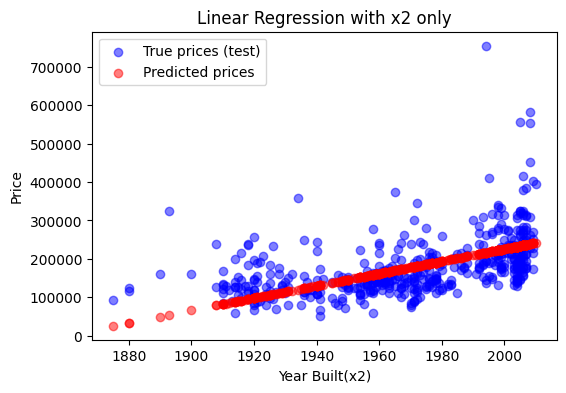
\includegraphics[width=0.6\textwidth]{../imgs/model_x2.png} % 
		\caption{Linear regression fit (x2)}
	\end{figure}

	\pagebreak
	\textbf{(x1,x2)}
	Error: 43,871.68
	\begin{figure}[h] % h = here, t = top, b = bottom
		\centering
		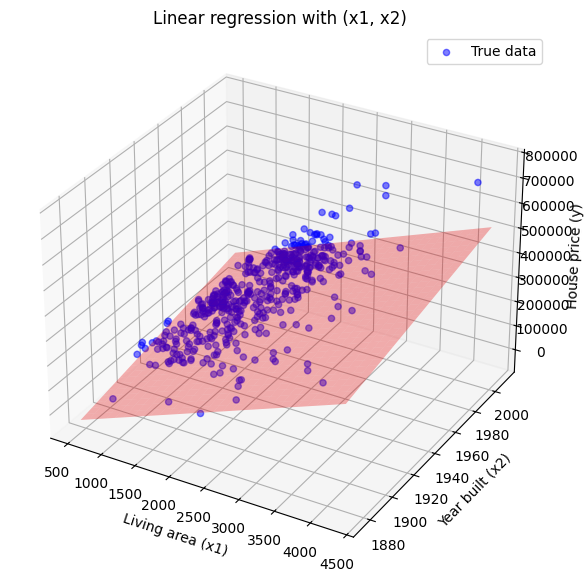
\includegraphics[width=0.6\textwidth]{../imgs/model_x1_x2.png} % 
		\caption{Linear regression fit (x1,x2)}
	\end{figure}

	\subsection{Part 2}
	We are now solving a non-linear polynomial regression compared to the previous linear regression models.

	The loss for this model is
	\[
		39{,}013.01
	\]
	which is lower than the loss of the linear model using \((x_1, x_2)\), given by
	\[
		43{,}871.68.
	\]

	\pagebreak

	\subsection*{3. Ridge Regression}

	The ridge regression solution is:
	\[
		w^{*} = (X^{\top}X + \lambda I)^{-1} X^{\top}y,
	\]

	where $\lambda$ is the regularization coefficient.

	We experiment with
	\[
		\lambda \in \{10^{-5},\, 10^{-4},\, 10^{-3},\, 10^{-2},\, 10^{-1}\}.
	\]

	\noindent \textbf{Results:}

	\begin{table}[h]
		\centering
		\begin{tabular}{c c}
			\hline
			$\lambda$          & Test Error    \\
			\hline
			$1 \times 10^{-5}$ & $60{,}833.94$ \\
			$1 \times 10^{-4}$ & $60{,}819.43$ \\
			$1 \times 10^{-3}$ & $60{,}676.10$ \\
			$1 \times 10^{-2}$ & $59{,}407.39$ \\
			$1 \times 10^{-1}$ & $54{,}314.09$ \\
			\hline
		\end{tabular}
		\caption{Ridge regression test errors for different values of $\lambda$.}
	\end{table}

	\begin{figure}[h] % h = here, t = top, b = bottom
		\centering
		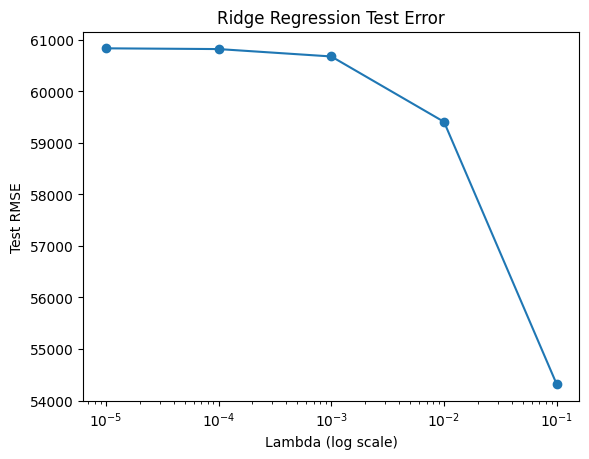
\includegraphics[width=0.6\textwidth]{../imgs/ridge-regression.png} % 
		\caption{Ridge regression error by lambda}
	\end{figure}


	For very small $\lambda$, the results are close to ordinary least squares.
	As $\lambda$ increases moderately, the test error decreases, suggesting better generalization.
	When $\lambda$ becomes too large, the model begins to underfit, leading to higher errors.
	The trend aligns with expectations: the error curve should take a U-shape, initially decreasing and then rising as $\lambda$
\end{homeworkProblem}

\pagebreak

\begin{homeworkProblem}

	\subsection{Part 1}

	For each training example $(x^{(i)}, y^{(i)})$ with $y^{(i)} \in \{0,1\}$, the model is
	\[
		f(x^{(i)}) = \sigma(w^\top \varphi(x^{(i)})), \quad
		\sigma(z) = \frac{1}{1+e^{-z}}.
	\]

	The likelihood of observing $y^{(i)}$ given $x^{(i)}$ is
	\[
		p(y^{(i)} \mid x^{(i)}, f(x^{(i)}))
		= \big(f(x^{(i)})\big)^{y^{(i)}} \, \big(1 - f(x^{(i)})\big)^{1-y^{(i)}}.
	\]

	The full likelihood over the dataset is
	\[
		L(w) = \prod_{i=1}^N \big(f(x^{(i)})\big)^{y^{(i)}} \, \big(1 - f(x^{(i)})\big)^{1-y^{(i)}}.
	\]

	The negative log-likelihood (NLL) is
	\[
		\ell(w) = - \sum_{i=1}^N \Big[ y^{(i)} \log f(x^{(i)}) + (1-y^{(i)}) \log (1-f(x^{(i)})) \Big].
	\]


	\subsection{Part 2}

	The gradient of $\ell(w)$ is
	\[
		\nabla \ell(w) = \sum_{i=1}^N \big(f(x^{(i)}) - y^{(i)}\big)\, \varphi(x^{(i)}).
	\]

	The Hessian is
	\[
		\nabla^2 \ell(w) = \sum_{i=1}^N f(x^{(i)})(1-f(x^{(i)}))\, \varphi(x^{(i)}) \varphi(x^{(i)})^\top.
	\]

	For any $v \in \mathbb{R}^M$,
	\[
		v^\top \nabla^2 \ell(w) v
		= \sum_{i=1}^N f(x^{(i)})(1-f(x^{(i)})) \, (v^\top \varphi(x^{(i)}))^2 \geq 0.
	\]

	Therefore, the Hessian is positive semidefinite and $\ell(w)$ is convex.

	\subsection{Part 3}

	The gradient descent update for $w$ is
	\[
		w \leftarrow w - \eta \, \nabla \ell(w),
	\]

	\[
    w^{(i)} = w^{(i-1)}- \epsilon \, \nabla \ell(w),
	\]
	where $\epsilon$ is the learning rate.

\end{homeworkProblem}

\end{document}
